% !TEX root = ./Cours.tex
\documentclass[../€Cours-complet/Cours-complet]{subfiles}

\usepackage{./figures}
\usetikzlibrary{calc,positioning}

\titleorchapter{Solides de l'espace, volume}{12}

\begin{document}

\maketitleCours

\section{Pavé droit}

\begin{cours}[Vocabulaire pavé droit]

	\begin{center}
		\newcommand{\rectWidth}{3}
		\newcommand{\rectHeight}{2}
		\begin{tikzpicture}
			\coordinate (A) at (0,0);
			\coordinate (B) at ($(A) + (\rectWidth,0)$);
			\coordinate (C) at ($(A) + (\rectWidth,\rectHeight)$);
			\coordinate (D) at ($(A) + (0,\rectHeight)$);

			\coordinate (E) at ($(A) + (1,1)$);
			\coordinate (F) at ($(E) + (\rectWidth,0)$);
			\coordinate (G) at ($(E) + (\rectWidth,\rectHeight)$);
			\coordinate (H) at ($(E) + (0,\rectHeight)$);

			\draw[ultra thin,fill=blue!30,draw=transparent] (B) -- (F) -- (G) -- (C) -- (B);

			\paveDroit{\rectHeight}{\rectWidth}{(1,1)}

			\foreach \p / \pos in {
					A/below left,
					B/below right,
					C/above left,
					D/above left,
					E/below,
					F/below right,
					G/above right,
					H/above} {
					\node[\pos] at (\p) {\p};
				}

			\draw[draw=green,ultra thick] (D) -- (H);
			\node at (A) {\color{red}∙};

			\draw[->] ($(A) - (2,0)$) node[left] {{\color{red}Sommet} A} -- ($(A) - (0.5,0)$);
			\draw[->] ($(D) + (-1,1.5)$) node[left] {{\color{green}Arête} [DH]} -- ($(D) + (0.3,0.7)$);
			\draw[->] ($(F) + (1,0.5)$) node[right] {{\color{blue}Face} BFGC} -- ($(F) + (-0.5,0.5)$);
		\end{tikzpicture}
	\end{center}

	\vspace{1em}
	La figure ci-dessus est un \textbf{pavé droit} (ou \textbf{parallélépipède rectangle}).
\end{cours}

\begin{cours}[Propriétés du pavé droit]
	Un pavé droit a
	\begin{itemize}
		\item \textbf{6 faces rectangulaires}.
		\item \textbf{12 arêtes}.
		\item \textbf{8 sommets}.
	\end{itemize}

	Le \textbf{volume $𝒱$} d'un parallélépipède rectangle de \uline{longueur} \textit{L}, de \uline{largeur} $𝑙$ et de \uline{hauteur} \textit{h} est :
	$$ 𝒱 = \textit{L} × l × \textit{h} $$
\end{cours}

\begin{exemple}
	Un pavé droit de longueur $10cm$, de largeur $5cm$ et de hauteur $20cm$ a un volume de
	\begin{align*}
		𝒱 & = 10cm × 5cm × 20cm                             \\
		  & = 1000cm³                                       \\
		  & = 1dm³              & \text{(1 décimètre cube)}
	\end{align*}
\end{exemple}

\begin{cours}[Patron du pavé droit]
	Le patron d'un pavé droit est

	\begin{center}
		\newcommand{\rectWidth}{2}
		\newcommand{\rectHeight}{1.2}
		\newcommand{\rectDepth}{2.5}
		\newcommand{\rectVraiWidth}{4cm}
		\newcommand{\rectVraiHeight}{3cm}
		\newcommand{\rectVraiDepth}{5cm}
		\newcommand{\patronX}{6}
		\newcommand{\patronY}{2}
		\begin{tikzpicture}
			\coordinate (A) at (0,0);
			\coordinate (B) at ($(A) + (\rectWidth,0)$);
			\coordinate (C) at ($(A) + (\rectWidth,\rectHeight)$);
			\coordinate (D) at ($(A) + (0,\rectHeight)$);

			\coordinate (E) at ($(A) + (1,1)$);
			\coordinate (F) at ($(E) + (\rectWidth,0)$);
			\coordinate (G) at ($(E) + (\rectWidth,\rectHeight)$);
			\coordinate (H) at ($(E) + (0,\rectHeight)$);

			\draw[ultra thin,fill=blue!30,draw=transparent] (B) -- (F) -- (G) -- (C) -- cycle;
			\draw[ultra thin,fill=red!30,draw=transparent] (D) -- (H) -- (G) -- (C) -- cycle;
			\draw[ultra thin,fill=green!30,draw=transparent] (D) -- (C) -- (B) -- (A) -- cycle;

			\draw[ultra thin] (B) -- (C) -- (D) -- (A) -- (B) -- (F) -- (G) -- (H) -- (D)
			(C) -- (G);
			\draw[thin,dotted] (E) -- (A)
			(E) -- (H)
			(E) -- (F);

			\draw[<->] ($(A) - (0,0.2)$) -- node[midway,below] {\rectVraiWidth} ($(B) - (0,0.2)$);
			\draw[<->] ($(A) - (0.2,0)$) -- node[midway,left] {\rectVraiHeight} ($(D) - (0.2,0)$);
			\draw[<->] ($(D) + (-0.15,0.15)$) -- node[midway,above left] {\rectVraiDepth} ($(H) + (-0.15,0.15)$);

			% Flèches
			\draw[very thick,purple,->] (3.5,1.5) -- ++(1,0);
			\draw[very thick,purple,->] (4.5,0.5) -- ++(-1,0);

			% Patron
			\draw[<->] (\patronX - 0.2,\patronY) -- node[midway,left] {\rectVraiDepth} ++(0,-\rectDepth);
			\draw[<->] (\patronX + \rectWidth + \rectHeight - 0.2,\patronY) -- node[midway,left] {\rectVraiHeight} ++(0,\rectHeight);
			\draw[<->] (\patronX + \rectWidth + \rectHeight,\patronY + \rectHeight + 0.2) -- node[midway,above] {\rectVraiWidth} ++(\rectWidth,0);

			\patronPaveDroit[fill=red!30][fill=blue!30][fill=green!30]{\rectHeight}{\rectWidth}{\rectDepth}[\patronX][\patronY]
		\end{tikzpicture}
	\end{center}
\end{cours}

\section{Cylindre}

\begin{cours}[Cylindre]
	\begin{center}
		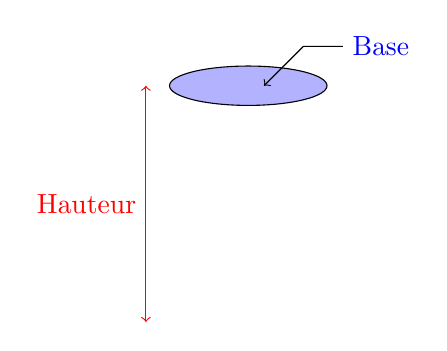
\begin{tikzpicture}
			\cylindre{3}{2}{0.5};
			\draw[draw=transparent,fill=blue!30] (0,0) ellipse (1 and 0.25);
			\draw[->] (1.2,0.5) node[right] {\color{blue}Base} -- ++(-0.5,0) -- ++(-0.5,-0.5);
			\draw[red,<->] (-1.3,0) -- node[midway,left] {\color{red}Hauteur} ++(0,-3);
		\end{tikzpicture}
	\end{center}

	La figure ci-dessus est un \textbf{cylindre}.

	Les deux disques sont les {\color{blue}\textbf{bases}} du cylindre. La longueur du segment reliant le centre des deux bases est la {\color{red}\textbf{hauteur}}.
\end{cours}

\begin{cours}[Propriétés du cylindre]
	Le \textbf{volume $𝒱$} d'un cylindre de \uline{hauteur} \textit{h} et dont le \uline{rayon} de la base est \textit{r} est :
	$$ 𝒱 = \text{π} × \textit{r} × \textit{r} × \textit{h} $$
\end{cours}

\begin{cours}[Patron du cylindre]
	Le patron d'un cylindre est

	\begin{center}
		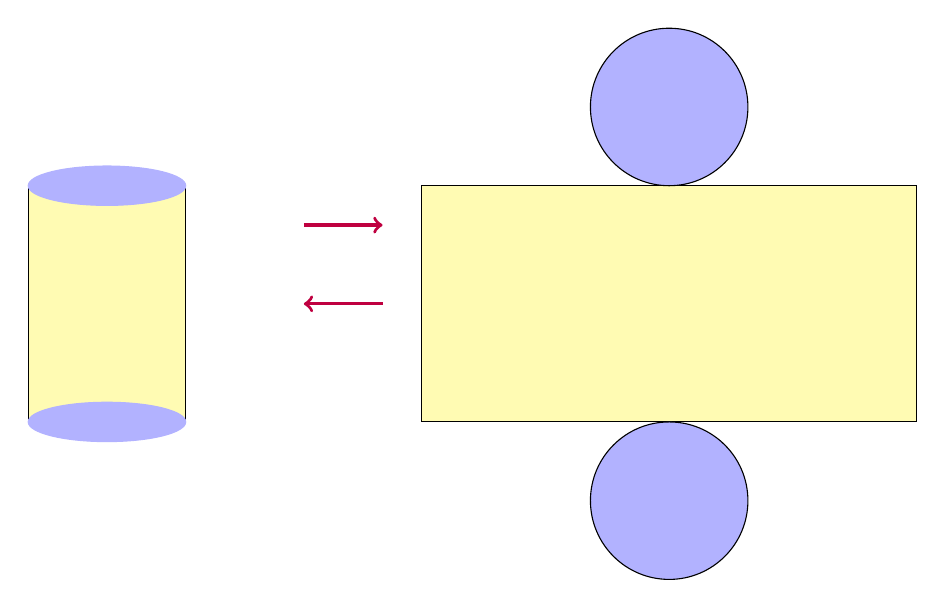
\begin{tikzpicture}
			\draw[draw=transparent,fill=yellow!30] (-1,0) -- ++(2,0) -- ++(0,-3) -- ++(-2,0) -- cycle;
			\draw[draw=blue!30,fill=blue!30] (0,0) ellipse (1 and 0.25);
			\draw[draw=blue!30,fill=blue!30] (0,-3) ellipse (1 and 0.25);
			\cylindre{3}{2}{0.5};

			% Flèches
			\draw[very thick,purple,->] (2.5,-0.5) -- ++(1,0);
			\draw[very thick,purple,->] (3.5,-1.5) -- ++(-1,0);

			% Patron
			\draw[fill=yellow!30] (4,0) -- ++(6.28,0) -- ++(0,-3) -- ++(-6.28,0) -- cycle;
			\draw[fill=blue!30] (7.14,1) circle (1);
			\draw[fill=blue!30] (7.14,-4) circle (1);
		\end{tikzpicture}
	\end{center}
\end{cours}

\section{Pyramide}

\section{Cône}

\end{document}